\documentclass[conference]{IEEEtran}
\IEEEoverridecommandlockouts
% The preceding line is only needed to identify funding in the first footnote. If that is unneeded, please comment it out.
%----------------------------------------------------------
\usepackage{cite}
\usepackage[pdftex]{graphicx}
% declare the path(s) where your graphic files are
\graphicspath{images/}
\DeclareGraphicsExtensions{.pdf,.jpeg,.png,.jpg}
\usepackage{amsmath,amssymb,amsfonts}
\usepackage{algorithmic}
\usepackage{graphicx}
\usepackage{textcomp}
\usepackage{array}
%\usepackage[caption=false,font=normalsize,labelfont=sf,textfon =sf]{subfig}
\usepackage{dblfloatfix}
\usepackage{url}
\usepackage{lipsum}
\usepackage{listings}
\usepackage{xcolor}
\def\BibTeX{{\rm B\kern-.05em{\sc i\kern-.025em b}\kern-.08em
    T\kern-.1667em\lower.7ex\hbox{E}\kern-.125emX}}
%----------------------------------------------------------
    \lstset{
        escapeinside={/*@}{@*/},
        language=Python,	
        basicstyle=\fontsize{8.5}{12}\selectfont,
        numbers=left,
        numbersep=2pt,    
        xleftmargin=2pt,
        frame=tb,
        columns=fullflexible,
        showstringspaces=false,
        tabsize=4,
        keepspaces=true,
        showtabs=false,
        showspaces=false,
        morekeywords={inline,public,class,private,protected,struct},
        captionpos=b,
        lineskip=-0.4em,
        aboveskip=10pt,
        extendedchars=true,
        breaklines=true,
        prebreak = \raisebox{0ex}[0ex][0ex]{\ensuremath{\hookleftarrow}},
        keywordstyle=\color[rgb]{0,0,1},
        commentstyle=\color[rgb]{0.133,0.545,0.133},
        stringstyle=\color[rgb]{0.627,0.126,0.941},
    }
%----------------------------------------------------------

\begin{document}

\title{Controle de braços robóticos auxiliados por visão computacional.
% \\
% {\footnotesize \textsuperscript{*} Sistemas Embarcados: Prof. Marco Reis - marco.reis@ba.docente.senai.brr}
% \thanks{Identify applicable funding agency here. If none, delete this.}
}

% \author{\IEEEauthorblockN{Marco Reis, 41650-010\IEEEauthorrefmark{1}}
% \IEEEauthorblockA{\IEEEauthorrefmark{1}Robotics & Autonomous Systems Center,
% Senai Cimatec, Salvador, Brazil}% <-this % stops an unwanted space


\author{\IEEEauthorblockN{Marco Reis}
\IEEEauthorblockA{\textit{SENAI CIMATEC} \\
% \textit{name of organization (of Aff.)}\\
Salvador, Brasil \\
marco.reis@aln.senaicimatec.edu.br}
\and
\IEEEauthorblockN{Icaro Borges de Macedo (orientador)}
\IEEEauthorblockA{\textit{SENAI CIMATEC} \\
% \textit{name of organization (of Aff.)}\\
Salvador, Brasil \\
icaro.macedo@fieb.org.br}
\and
\IEEEauthorblockN{Tiago Barretto Sant’Anna}
\IEEEauthorblockA{\textit{SENAI CIMATEC} \\
% \textit{name of organization (of Aff.)}\\
Salvador, Brasil\\
tiago.sant'anna@ba.estudante.senai.br}
\and
\IEEEauthorblockN{Samuel Luiz Silva Santana }
\IEEEauthorblockA{\textit{SENAI CIMATEC} \\
% \textit{name of organization (of Aff.)}\\
Salvador, Brasil \\
samuel.santana@ba.estudante.senai.br}
\and
% \IEEEauthorblockN{5\textsuperscript{th} Given Name Surname}
% \IEEEauthorblockA{\textit{dept. name of organization (of Aff.)} \\
% % \textit{name of organization (of Aff.)}\\
% City, Country \\
% email address or ORCID}
% \and
% \IEEEauthorblockN{6\textsuperscript{th} Given Name Surname}
% \IEEEauthorblockA{\textit{dept. name of organization (of Aff.)} \\
% \textit{name of organization (of Aff.)}\\
% City, Country \\
% email address or ORCID}
}

\maketitle

\begin{abstract}
O objetivo deste artigo é expor os problemas na automação dentro da área da robótica industrial e trabalhar para consertar esse fato. Portanto visando tornar a tecnologia robótica mais autônoma, mais especificamente os braços robóticos, desenvolvemos esse artigo que visa interromper a dependência de uma programação que limita esses robôs a fazer apenas movimentos repetitivos com peças específicas sem nenhuma capacidade de realizar outros movimentos além daqueles pré-programados. Sabemos que esse é um problema que depende de um grande acúmulo de conhecimento antes de poder ser solucionado, devido a esse fato decidimos realizar pesquisas sobre o assunto e desenvolver resultados utilizando a visão computacional. Esses resultados devem impactar diretamente no dia-a-dia da indústria, pois irá reduzir a necessidade de programar novamente um robô para cada mudança em sua função.
\end{abstract}

\begin{IEEEkeywords}
robótica, mecatrônica, manipuladores, visão computacional.
\end{IEEEkeywords}

\section{Introduction}

A robótica é uma área em crescimento no mundo, podendo se expandir até 10 vezes mais na última década \cite{Roboticonline}. Esse aumento se dá principalmente na indústria, onde o uso da robótica gera um maior aumento da produtividade \cite{robotica1}. Desse modo, é uma área que necessita de constantes avanços tecnológicos para suprir essa demanda. Porém, um problema encontrado na robótica industrial é que sua automação não consegue ser independente o suficiente. Quando se programa um braço robótico ele pode fazer o mesmo movimento diversas vezes de forma autônoma, entretanto caso a peça a ser manipulada seja deslocada, o braço não tem capacidade, de forma autônoma, de alterar sua trajetória para poder trabalhar com ela. Assim, como fazer com que um braço robótico possa pegar objetos específicos, independente de suas posições no espaço? Dessa maneira, o objetivo desse artigo é estudar e criar um braço robótico cuja função é coletar objetos, independente de qual posição eles estejam, fazendo o uso de visão computacional. Os objetivos específicos desse artigo, são o estudo e geração do reconhecimento de peças com visão computacional, a cinemática do manipulador, a programação do manipulador e a integração da câmera com o braço robótico.  A importância desse procedimento tem como consequência uma diminuição na necessidade de reprogramação desses braços robóticos, irá facilitar a programação para poder realizar tarefas ainda mais complexas, fornecendo assim economia e efetividade. Dessa forma será realizada uma pesquisa bibliográfica, acerca de braços robóticos, visão computacional e cinemática. Esse trabalho é uma pesquisa aplicada, com objetivo exploratório, por uma abordagem qualitativa.

\section{Fundamentação teórica}

\subsection{Identificação de objetos}

Para poder fazer a identificação dos objetos foram escolhidos fazer o uso de marco fiduciais. Esses marcos fiduciais são imagens ou objetos usados como pontos de referencia para os robôs realizarem certas ações \cite{Fiducial26:online}. % Change this reference later, not use wikipedia.
Com o uso desses marcadores, facilitará na hora de identificar a posição dos objeto no espaço e sua orientação.


\begin{figure}[h!]
\centering
    
\includegraphics[width=4cm]{images/markers.jpg}
\caption{Exemplos de tags \cite{OpenCVDe76:online}}
\label{fig:tags}
\end{figure}

A figura \ref{fig:tags} mostra um exemplo dessas tags. Elas possuem padrões que são facilmente identificados pelas cameras e se dado as suas dimensões pode se usar algoritmos para descobrir suas coordenadas no espaço. Dessa forma foi pensado em colocar uma camera em uma posição estratégica do braço para dar uma melhor visão dos objetos e poder reconhece-los, além de usar sua posição para definir a cinemática do braço.

\begin{figure}[h!]
    \centering
        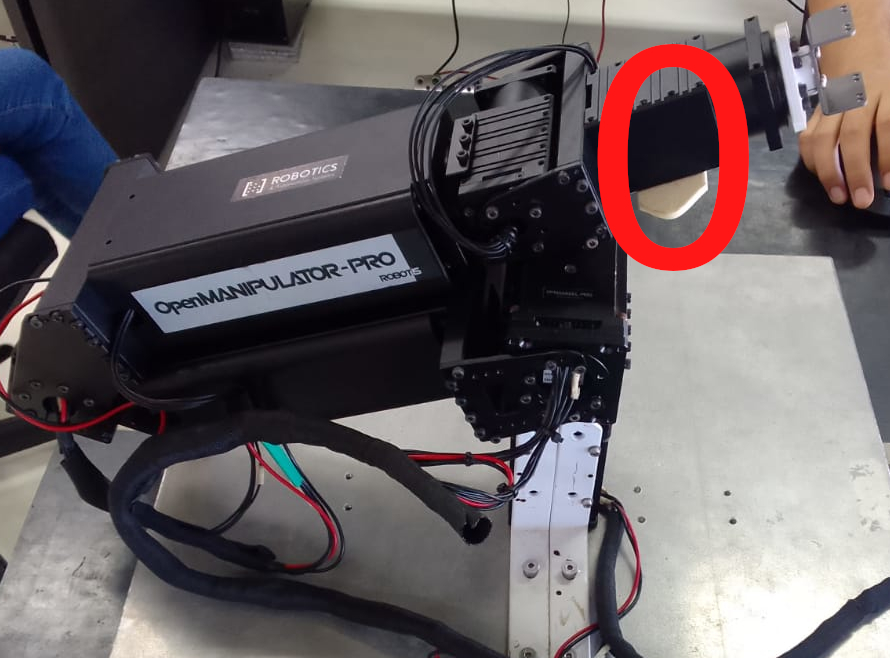
\includegraphics[width=8cm]{images/arm_marked.jpeg}
    \caption{Imagem do braço robótico}
    \label{fig:cam_arm}
\end{figure}

Por questão de praticidade foi decidido usar uma webcam para captar as imagens do ambiente, essa camera sera colocada na parte sinalizada no braço robótico, explicitado na figura \ref{fig:cam_arm}. Assim será processado para onde a ferramenta esta direcionada.

\subsubsection{Calibração da camera}

A calibração é uma parte fundamental para conseguir parâmetros fundamentais de uma camera, com esses dados se consegue determinar onde esta um ponto 3D no espaço \cite{ArUco}. Isso é feito para obter valores, como o de pixels da camera, coeficientes de distorção e centro óptico do sensor \cite{ArUco}.

\begin{figure}[h!]
    \centering
        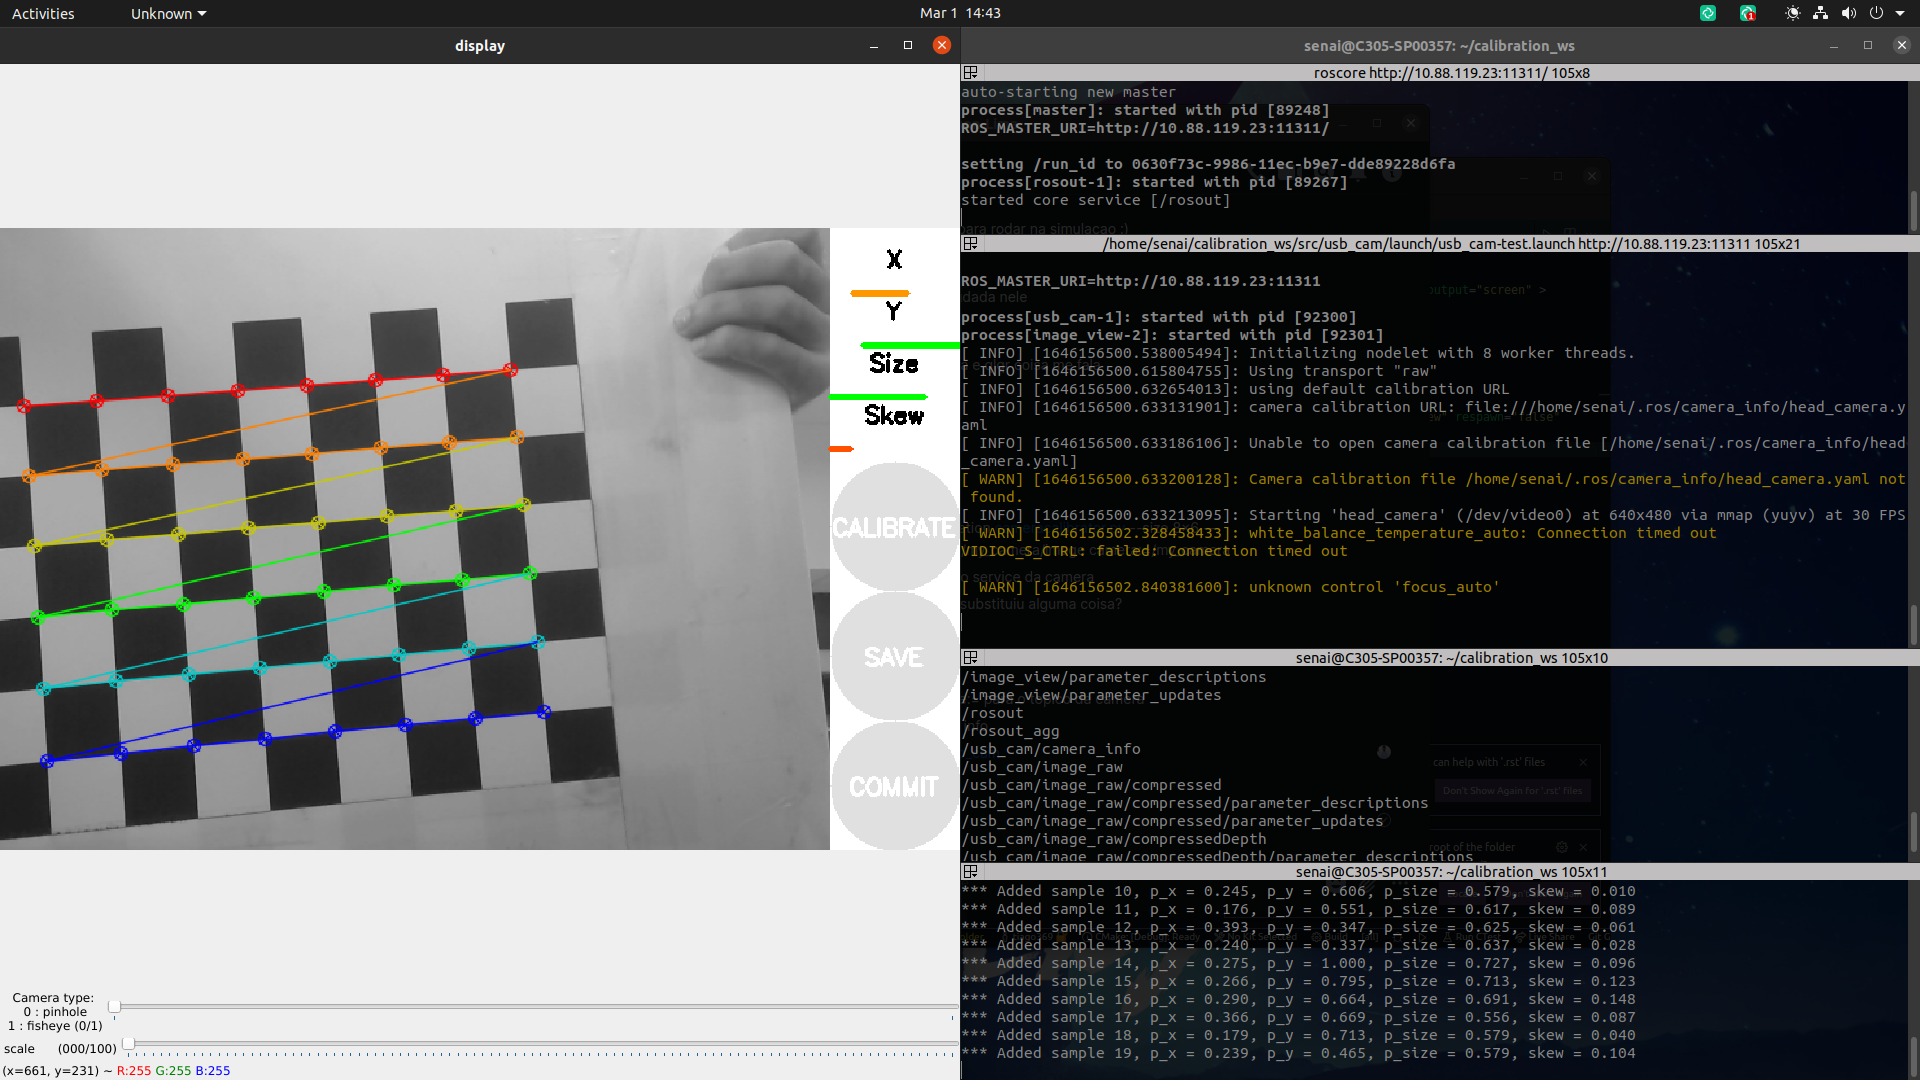
\includegraphics[width=9cm]{images/calibration.png}
    \caption{Calibração}
    \label{fig:calibration}
\end{figure}

Dessa forma a calibração foi feita usando o \textit{ROS Noetic}, com um pacote especifico para calibração \cite{camera_calibration:online} e um pacote próprio para conectar a webcam no pc \cite{usbcamRO60:online}. Parte do processo da calibração pode ser mostrado na imagem \ref{fig:calibration}. Com esse processo foi gerado um arquivo comprimido com todas as informações necessárias para configurar a camera. Assim foi finalizado essa etapa do processo

% -------------------------------------------------------------------
\section{Prepare Your Paper Before Styling}
Before you begin to format your paper, first write and save the content as a 
separate text file. Complete all content and organizational editing before 
formatting. Please note sections \ref{AA}--\ref{SCM} below for more information on 
proofreading, spelling and grammar.

Keep your text and graphic files separate until after the text has been 
formatted and styled. Do not number text heads---{\LaTeX} will do that 
for you.

\subsection{Abbreviations and Acronyms}\label{AA}
Define abbreviations and acronyms the first time they are used in the text, 
even after they have been defined in the abstract. Abbreviations such as 
IEEE, SI, MKS, CGS, ac, dc, and rms do not have to be defined. Do not use 
abbreviations in the title or heads unless they are unavoidable.

\subsection{Units}
\begin{itemize}
\item Use either SI (MKS) or CGS as primary units. (SI units are encouraged.) English units may be used as secondary units (in parentheses). An exception would be the use of English units as identifiers in trade, such as ``3.5-inch disk drive''.
\item Avoid combining SI and CGS units, such as current in amperes and magnetic field in oersteds. This often leads to confusion because equations do not balance dimensionally. If you must use mixed units, clearly state the units for each quantity that you use in an equation.
\item Do not mix complete spellings and abbreviations of units: ``Wb/m\textsuperscript{2}'' or ``webers per square meter'', not ``webers/m\textsuperscript{2}''. Spell out units when they appear in text: ``. . . a few henries'', not ``. . . a few H''.
\item Use a zero before decimal points: ``0.25'', not ``.25''. Use ``cm\textsuperscript{3}'', not ``cc''.)
\end{itemize}

\subsection{Equations}
Number equations consecutively. To make your 
equations more compact, you may use the solidus (~/~), the exp function, or 
appropriate exponents. Italicize Roman symbols for quantities and variables, 
but not Greek symbols. Use a long dash rather than a hyphen for a minus 
sign. Punctuate equations with commas or periods when they are part of a 
sentence, as in:
\begin{equation}
a+b=\gamma\label{eq}
\end{equation}

Be sure that the 
symbols in your equation have been defined before or immediately following 
the equation. Use ``\eqref{eq}'', not ``Eq.~\eqref{eq}'' or ``equation \eqref{eq}'', except at 
the beginning of a sentence: ``Equation \eqref{eq} is . . .''

\subsection{\LaTeX-Specific Advice}

Please use ``soft'' (e.g., \verb|\eqref{Eq}|) cross references instead
of ``hard'' references (e.g., \verb|(1)|). That will make it possible
to combine sections, add equations, or change the order of figures or
citations without having to go through the file line by line.

Please don't use the \verb|{eqnarray}| equation environment. Use
\verb|{align}| or \verb|{IEEEeqnarray}| instead. The \verb|{eqnarray}|
environment leaves unsightly spaces around relation symbols.

Please note that the \verb|{subequations}| environment in {\LaTeX}
will increment the main equation counter even when there are no
equation numbers displayed. If you forget that, you might write an
article in which the equation numbers skip from (17) to (20), causing
the copy editors to wonder if you've discovered a new method of
counting.

{\BibTeX} does not work by magic. It doesn't get the bibliographic
data from thin air but from .bib files. If you use {\BibTeX} to produce a
bibliography you must send the .bib files. 

{\LaTeX} can't read your mind. If you assign the same label to a
subsubsection and a table, you might find that Table I has been cross
referenced as Table IV-B3. 

{\LaTeX} does not have precognitive abilities. If you put a
\verb|\label| command before the command that updates the counter it's
supposed to be using, the label will pick up the last counter to be
cross referenced instead. In particular, a \verb|\label| command
should not go before the caption of a figure or a table.

Do not use \verb|\nonumber| inside the \verb|{array}| environment. It
will not stop equation numbers inside \verb|{array}| (there won't be
any anyway) and it might stop a wanted equation number in the
surrounding equation.

\subsection{Some Common Mistakes}\label{SCM}
\begin{itemize}
\item The word ``data'' is plural, not singular.
\item The subscript for the permeability of vacuum $\mu_{0}$, and other common scientific constants, is zero with subscript formatting, not a lowercase letter ``o''.
\item In American English, commas, semicolons, periods, question and exclamation marks are located within quotation marks only when a complete thought or name is cited, such as a title or full quotation. When quotation marks are used, instead of a bold or italic typeface, to highlight a word or phrase, punctuation should appear outside of the quotation marks. A parenthetical phrase or statement at the end of a sentence is punctuated outside of the closing parenthesis (like this). (A parenthetical sentence is punctuated within the parentheses.)
\item A graph within a graph is an ``inset'', not an ``insert''. The word alternatively is preferred to the word ``alternately'' (unless you really mean something that alternates).
\item Do not use the word ``essentially'' to mean ``approximately'' or ``effectively''.
\item In your paper title, if the words ``that uses'' can accurately replace the word ``using'', capitalize the ``u''; if not, keep using lower-cased.
\item Be aware of the different meanings of the homophones ``affect'' and ``effect'', ``complement'' and ``compliment'', ``discreet'' and ``discrete'', ``principal'' and ``principle''.
\item Do not confuse ``imply'' and ``infer''.
\item The prefix ``non'' is not a word; it should be joined to the word it modifies, usually without a hyphen.
\item There is no period after the ``et'' in the Latin abbreviation ``et al.''.
\item The abbreviation ``i.e.'' means ``that is'', and the abbreviation ``e.g.'' means ``for example''.
\end{itemize}
An excellent style manual for science writers is \cite{young1989technical}.

\subsection{Authors and Affiliations}
\textbf{The class file is designed for, but not limited to, six authors.} A 
minimum of one author is required for all conference articles. Author names 
should be listed starting from left to right and then moving down to the 
next line. This is the author sequence that will be used in future citations 
and by indexing services. Names should not be listed in columns nor group by 
affiliation. Please keep your affiliations as succinct as possible (for 
example, do not differentiate among departments of the same organization).

\subsection{Identify the Headings}
Headings, or heads, are organizational devices that guide the reader through 
your paper. There are two types: component heads and text heads.

Component heads identify the different components of your paper and are not 
topically subordinate to each other. Examples include Acknowledgments and 
References and, for these, the correct style to use is ``Heading 5''. Use 
``figure caption'' for your Figure captions, and ``table head'' for your 
table title. Run-in heads, such as ``Abstract'', will require you to apply a 
style (in this case, italic) in addition to the style provided by the drop 
down menu to differentiate the head from the text.

Text heads organize the topics on a relational, hierarchical basis. For 
example, the paper title is the primary text head because all subsequent 
material relates and elaborates on this one topic. If there are two or more 
sub-topics, the next level head (uppercase Roman numerals) should be used 
and, conversely, if there are not at least two sub-topics, then no subheads 
should be introduced.

\subsection{Figures and Tables}
\paragraph{Positioning Figures and Tables} Place figures and tables at the top and 
bottom of columns. Avoid placing them in the middle of columns. Large 
figures and tables may span across both columns. Figure captions should be 
below the figures; table heads should appear above the tables. Insert 
figures and tables after they are cited in the text. Use the abbreviation 
``Fig.~\ref{fig}'', even at the beginning of a sentence.

\begin{table}[htbp]
\caption{Table Type Styles}
\begin{center}
\begin{tabular}{|c|c|c|c|}
\hline
\textbf{Table}&\multicolumn{3}{|c|}{\textbf{Table Column Head}} \\
\cline{2-4} 
\textbf{Head} & \textbf{\textit{Table column subhead}}& \textbf{\textit{Subhead}}& \textbf{\textit{Subhead}} \\
\hline
copy& More table copy$^{\mathrm{a}}$& &  \\
\hline
\multicolumn{4}{l}{$^{\mathrm{a}}$Sample of a Table footnote.}
\end{tabular}
\label{tab1}
\end{center}
\end{table}

\begin{figure}[htbp]
\centerline{
    \includegraphics{images/fig1.png}
    }
\caption{Example of a figure caption.}
\label{fig}
\end{figure}

Figure Labels: Use 8 point Times New Roman for Figure labels. Use words 
rather than symbols or abbreviations when writing Figure axis labels to 
avoid confusing the reader. As an example, write the quantity 
``Magnetization'', or ``Magnetization, M'', not just ``M''. If including 
units in the label, present them within parentheses. Do not label axes only 
with units. In the example, write ``Magnetization (A/m)'' or ``Magnetization 
\{A[m(1)]\}'', not just ``A/m''. Do not label axes with a ratio of 
quantities and units. For example, write ``Temperature (K)'', not 
``Temperature/K''.


\section*{Acknowledgment}

The preferred spelling of the word ``acknowledgment'' in America is without an ``e'' after the ``g''. Avoid the stilted expression ``one of us (R. B. G.) thanks $\ldots$''. Instead, try ``R. B. G. thanks$\ldots$''. Put sponsor acknowledgments in the unnumbered footnote on the first page.

\section*{References}

Please number citations consecutively within brackets \cite{eason1955certain}.
The sentence punctuation follows the bracket \cite{clerk1892maxwell}. Refer simply to the reference number, as in \cite{jacobs1963fine}---do not use ``Ref. \cite{jacobs1963fine}'' or ``reference \cite{jacobs1963fine}'' except at 
the beginning of a sentence: ``Reference \cite{jacobs1963fine} was the first $\ldots$''

Number footnotes separately in superscripts. Place the actual footnote at 
the bottom of the column in which it was cited. Do not put footnotes in the 
abstract or reference list. Use letters for table footnotes.

Unless there are six authors or more give all authors' names; do not use 
``et al.''. Papers that have not been published, even if they have been 
submitted for publication, should be cited as ``unpublished'' \cite{nicoletitle}. Papers 
that have been accepted for publication should be cited as ``in press'' \cite{elissatitle}. 
Capitalize only the first word in a paper title, except for proper nouns and 
element symbols.

For papers published in translation journals, please give the English 
citation first, followed by the original foreign-language citation \cite{yorozu1987electron}.

%----------------------------------------------------------
\bibliographystyle{IEEEtran}
\bibliography{Bibliography}
%CRITICAL: do not change the above two lines!!!
%----------------------------------------------------------

% \vspace{12pt}
% \color{red}
% Course templates contain guidance text for composing and formatting Course papers. Please ensure that all template text is removed from your course paper prior to submission to the lecturer. Failure to remove the template text from your paper may result in your paper not being accepted.

\end{document}
